\documentclass[12pt]{article}
\usepackage[dvipsnames]{xcolor}
\usepackage{tikz}
\usepackage{pdflscape}

\pagestyle{empty}
\begin{document}
\begin{landscape}
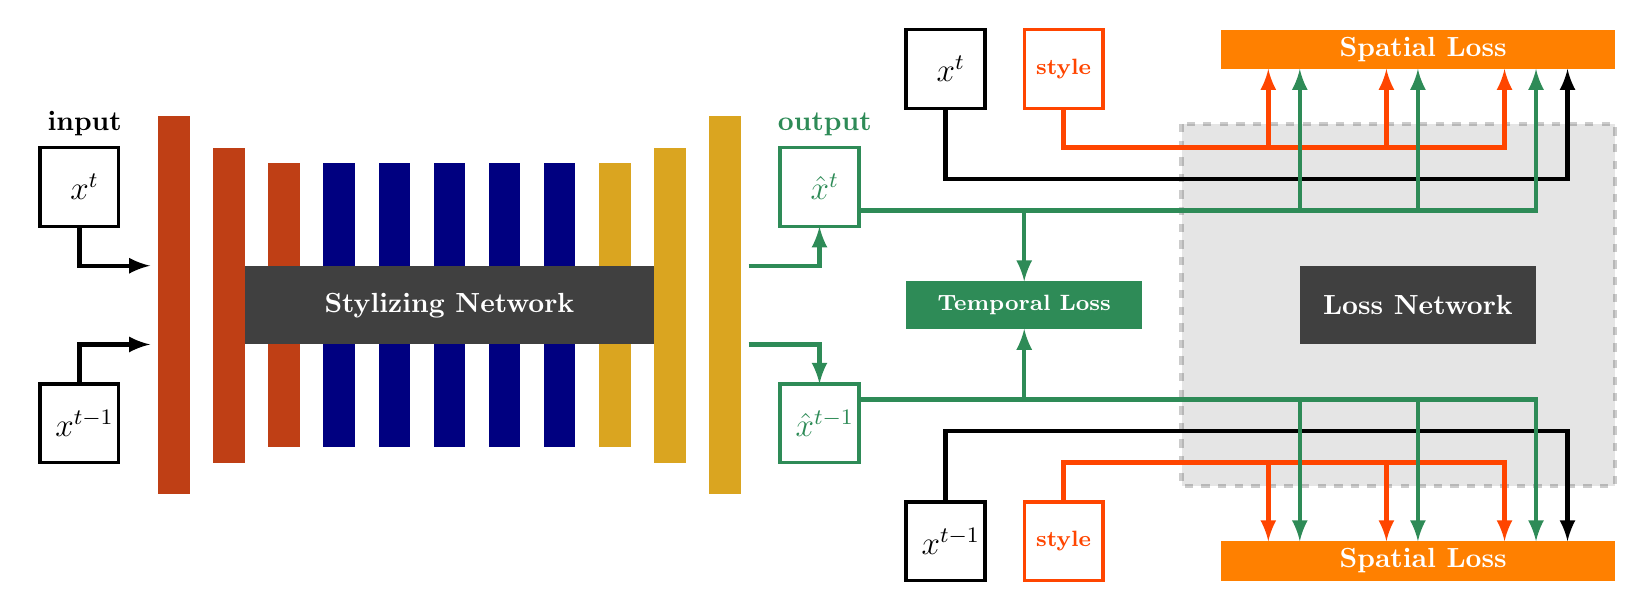
\begin{tikzpicture}
\centering
% Input
\draw (0.5,2.3) node {\textbf{ input}} ;
\draw[black,very thick](0,1) rectangle (1,2)node[pos=.5]{\textbf{ \large $x^t$}};
\draw[-latex,ultra thick, black] (0.5,1)--(0.5,0.5)--(1.4,0.5); 

\draw[black,very thick](0,-1) rectangle (1,-2)node[pos=.5]{\textbf{ \large $x^{t-1}$}};
\draw[-latex,ultra thick, black] (0.5,-1)--(0.5,-0.5)--(1.4,-0.5); 


% stylizing network
\fill[Bittersweet] (1.5,2.4) rectangle (1.9,-2.4);
\fill[Bittersweet] (2.2,2) rectangle (2.6,-2);
\fill[Bittersweet] (2.9,1.8) rectangle (3.3,-1.8);

\fill[NavyBlue] (3.6,1.8) rectangle (4,-1.8);
\fill[NavyBlue] (4.3,1.8) rectangle (4.7,-1.8);
\fill[NavyBlue] (5,1.8) rectangle (5.4,-1.8);
\fill[NavyBlue] (5.7,1.8) rectangle (6.1,-1.8);
\fill[NavyBlue] (6.4,1.8) rectangle (6.8,-1.8);

\fill[Goldenrod,fill opacity=1] (7.1,1.8) rectangle (7.5,-1.8);
\fill[Goldenrod,fill opacity=1] (7.8,2) rectangle (8.2,-2);
\fill[Goldenrod,fill opacity=1] (8.5,2.4) rectangle (8.9,-2.4);

\fill[darkgray,fill opacity=1,text=white] (2.6,0.5) rectangle (7.8,-0.5)node[pos=.5] {\textbf{Stylizing Network}};

% Output
\draw (9.9,2.3) node [SeaGreen]{\textbf{ output}} ;
\draw[SeaGreen,very thick](9.4,1) rectangle (10.4,2)node[pos=.5]{\textbf{ \large $\hat{x}^t$}};
\draw[-latex,ultra thick, SeaGreen] (9,0.5)--(9.9,0.5)--(9.9,1); 

\draw[SeaGreen,very thick](9.4,-1) rectangle (10.4,-2)node[pos=.5]{\textbf{ \large $\hat{x}^{t-1}$}};
\draw[-latex,ultra thick, SeaGreen] (9,-0.5)--(9.9,-0.5)--(9.9,-1); 

% Loss Network
\draw[dashed,ultra thick,black, opacity=0.2] (14.5,2.3) rectangle (20,-2.3);
\fill[black,fill opacity=0.1,text=white] (14.5,2.3) rectangle (20,-2.3);
\fill[darkgray,fill opacity=1,text=white] (16,0.5) rectangle (19,-0.5)node[pos=.5] {\textbf{Loss Network}};

% Temporal Loss
\draw[OrangeRed,very thick](12.5,2.5) rectangle (13.5,3.5)node[pos=.5]{\footnotesize\textbf{style}};
\draw[-latex,ultra thick, OrangeRed] (13,2.5)--(13,2)--(18.6,2)--(18.6,3); 
\draw[-latex,ultra thick, OrangeRed] (17.1,2)--(17.1,3); 
\draw[-latex,ultra thick, OrangeRed] (15.6,2)--(15.6,3); 

\draw[OrangeRed,very thick](12.5,-2.5) rectangle (13.5,-3.5)node[pos=.5]{\footnotesize\textbf{style}};
\draw[-latex,ultra thick, OrangeRed] (13,-2.5)--(13,-2)--(18.6,-2)--(18.6,-3); 
\draw[-latex,ultra thick, OrangeRed] (17.1,-2)--(17.1,-3); 
\draw[-latex,ultra thick, OrangeRed] (15.6,-2)--(15.6,-3); 


\draw[black,very thick](11,2.5) rectangle (12,3.5)node[pos=.5]{\textbf{ \large $x^t$}};
\draw[-latex,ultra thick, black] (11.5,2.5)--(11.5,1.6)--(19.4,1.6)--(19.4,3); 
\draw[black,very thick](11,-2.5) rectangle (12,-3.5)node[pos=.5]{\textbf{ \large $x^{t-1}$}};
\draw[-latex,ultra thick, black] (11.5,-2.5)--(11.5,-1.6)--(19.4,-1.6)--(19.4,-3); 


\fill[SeaGreen,text=white] (11,0.3) rectangle (14,-0.3)node[pos=.5] {\footnotesize{\textbf{Temporal Loss}}};
\draw[-latex,ultra thick, SeaGreen] (10.4,1.2)--(16,1.2)--(16,3); 
\draw[-latex,ultra thick, SeaGreen] (16,1.2)--(17.5,1.2)--(17.5,3); 
\draw[-latex,ultra thick, SeaGreen] (17.5,1.2)--(19,1.2)--(19,3); 
\draw[-latex,ultra thick, SeaGreen] (12.5,1.2)--(12.5,0.3); 

\draw[-latex,ultra thick, SeaGreen] (10.4,-1.2)--(16,-1.2)--(16,-3); 
\draw[-latex,ultra thick, SeaGreen] (16,-1.2)--(17.5,-1.2)--(17.5,-3); 
\draw[-latex,ultra thick, SeaGreen] (17.5,-1.2)--(19,-1.2)--(19,-3); 
\draw[-latex,ultra thick, SeaGreen] (12.5,-1.2)--(12.5,-0.3); 

%Spatial Loss
\fill[orange,text=white] (15,3) rectangle (20,3.5)node[pos=.5] {\textbf{ Spatial Loss}};
\fill[orange,text=white] (15,-3) rectangle (20,-3.5)node[pos=.5] {\textbf{ Spatial Loss}};


\end{tikzpicture}

\end{landscape}

\end{document} 